
\section{克鲁尔定理}

下面我们将引入一批将要反复使用的结果，它们把函数与其消失之处——那些余维数为 $1$ 的点——联系起来。关键的结果是\trKrull{}\trPrincipalIdealTheorem（Principal Ideal Theorem）：它在几何上令人可信，而其证明虽短，却又莫名地不直观而代数化。本节将需要\trNoetherian{}假设。

\textbf{12.3.1.\ \trKrull{}\trPrincipalIdealTheorem。}\quad 在一个\trVectorSpace{}中，单独一个线性方程切出的子空间，其\trCodimension{}总是 $0$ 或 $1$（且\trCodimension{}为 $0$ 仅当方程本身就是 $0$）。\trPrincipalIdealTheorem{}归功于 W.~\trKrull，它推广了这条线性代数事实。

\textbf{12.3.2.\ \trKrull{}\trPrincipalIdealTheorem（几何版本）。}\ ——\ \emph{设 $X$ 是一个\trLocally\trNoetherian\trScheme，$f$ 是一个函数。那么 $V(f)$ 的诸\trIrreducibleComponent{}的\trCodimension{}都是 $0$ 或 $1$。}

这显然是下面这条代数陈述的推论。

\textbf{12.3.3.\ \trKrull{}\trPrincipalIdealTheorem（代数版本）。}\ ——\ \emph{设 $A$ 是一个\trNoetherian{}环，$f\in A$。那么，凡在含 $f$ 的诸\trPrimeIdeal{}之中极小的 $\mathfrak{p}$，其\trCodimension{}至多为 $1$。再者，若 $f$ 不是\trZerodivisor，则每个含 $f$ 的这种 $\mathfrak{p}$，其\trCodimension{}都恰为 $1$。}

例如，\trLocallyPrincipal{}闭子概形具有「余维数 $0$ 或 $1$」，而\trEffectiveCartierDivisor{}具有「纯余维数 $1$」。下面是另一个例子（不用\trPrincipalIdealTheorem{}你当然也能直接证明它）。

\textbf{12.3.A.（练习）}\quad 证明：域 $k$ 上 $n+1$ 个变量的一个\trIrreducible\trHomogeneous{}多项式，描述 $\mathbb{P}^n_k$ 中一个\trDimension{}为 $n-1$ 的\trIntegral\trScheme。

你只须留意\trhTheorem{}~12.3.3 的证明有多短，然后径直跳到 \S12.3.5；等你把这个定理用得足够多、深切体会到它的价值之后，再回头读证明不迟。

\textbf{12.3.4.}\ \extrahard\ \textbf{\trKrull{}\trPrincipalIdealTheorem~12.3.3 之证明。}\quad 我们先料理最后一句：若 $\mathfrak{p}$ 的\trCodimension{}为 $0$，则它是一个\trAssociatedPrimeIdeal（\mbox{练习~6.6.M}），从而它的任何元素（包括 $f$ 在内）都是\trZerodivisor（命题~6.6.13）。

接下来我们要证 $\operatorname{codim}\mathfrak{p}\le1$。我们化归到局部环的情形：把 $A$ 换成 $A_{\mathfrak{p}}$（并把 $\mathfrak{p}$ 换成 $\mathfrak{p}A_{\mathfrak{p}}$）并不改变问题，故可设 $\mathfrak{p}$ 是一个\trMaximalIdeal。

反设 $\mathfrak{q}$ 是 $A$ 的一个严格更小的\trPrimeIdeal（于是由 $\mathfrak{p}$ 在含 $f$ 的诸\trPrimeIdeal{}之中的极小性，$f\notin\mathfrak{q}$）。我们要证 $\mathfrak{q}$ 的\trCodimension{}为 $0$。

证明的关键想法是下面这个巧妙的构造。

\textbf{12.3.B.（练习）}\quad 设 $\phi\colon A\to A_{\mathfrak{q}}$ 是\trLocalization，并定义 $\mathfrak{q}^{(n)}:=\phi^{-1}(\mathfrak{q}^nA_{\mathfrak{q}})$。（它称为 $\mathfrak{q}$ 的第 $n$ 个\textbf{\trSymbolicPower}（symbolic power），但我们不会使用这个术语。）注意 $\mathfrak{q}^{(1)}\supset\mathfrak{q}^{(2)}\supset\cdots$ 是 $A$ 的理想的一个降序列。若 $ag\in\mathfrak{q}^{(n)}$ 而 $g\notin\mathfrak{q}$，证明 $a\in\mathfrak{q}^{(n)}$。（转述：$\mathfrak{q}^{(n)}$ 是 $\mathfrak{q}$-\trPrimary{}的，尽管这个术语我们同样不去用它。）

现在 $\sqrt{(f)}\subset A$ 是含 $f$ 的诸\trMinimalPrimeIdeal{}之交（\cref{ex:radical-intersection-primes}），而这个交恰恰就是\trMaximalIdeal{} $\mathfrak{p}$。于是在局部环 $A/(f)$ 中，\trNilradical{}理想正是\trMaximalIdeal，故由命题~12.1.9（关于\trDimension{}为 $0$ 的\trNoetherian{}局部环），$A/(f)$ 的理想的任何降链都最终恒定。特别地，$\mathfrak{q}^{(1)}\supset\mathfrak{q}^{(2)}\supset\cdots$ 在 $A/(f)$ 中的像最终恒定，于是
\begin{equation*}\tag{12.3.4.1}\label{eq:symbolic-power-congruence}
\mathfrak{q}^{(n)}\equiv\mathfrak{q}^{(n+1)}\pmod{f}\qquad\text{对充分大的 }n\ge n_0.
\end{equation*}
接下来我们断言：事实上对 $n\ge n_0$ 有 $\mathfrak{q}^{(n)}=\mathfrak{q}^{(n+1)}+f\mathfrak{q}^{(n)}$。理由：设 $b_n\in\mathfrak{q}^{(n)}$。那么由式~\eqref{eq:symbolic-power-congruence}，$b_n=b_{n+1}+af$，其中 $b_{n+1}\in\mathfrak{q}^{(n+1)}\subset\mathfrak{q}^{(n)}$，而 $a\in A$。于是 $af\in\mathfrak{q}^{(n)}$；但 $f\notin\mathfrak{q}$。由\mbox{练习~12.3.B}，$a\in\mathfrak{q}^{(n)}$，故正如所断言的，$\mathfrak{q}^{(n)}=\mathfrak{q}^{(n+1)}+f\mathfrak{q}^{(n)}$。

于是，由\trNakayama{}引理~8.2.9（取 $A$，$M=\mathfrak{q}^{(n)}/\mathfrak{q}^{(n+1)}$，$I=(f)$），得 $\mathfrak{q}^{(n)}=\mathfrak{q}^{(n+1)}$，从而 $\mathfrak{q}^nA_{\mathfrak{q}}=\mathfrak{q}^{n+1}A_{\mathfrak{q}}$。再由\trNakayama{}引理~8.2.9（取 $A_{\mathfrak{q}}$，$M=\mathfrak{q}^nA_{\mathfrak{q}}$，$I=\mathfrak{q}A_{\mathfrak{q}}$），得 $\mathfrak{q}^nA_{\mathfrak{q}}=0$，故由命题~12.1.9，$A_{\mathfrak{q}}$ 的\trDimension{}为 $0$，从而 $\mathfrak{q}$ 在 $A$ 中的\trCodimension{}为 $0$，正如所愿。\hfill$\square$

\textbf{12.3.5.}\quad 现在我们用\trKrull{}\trPrincipalIdealTheorem{}来证明几条几何事实。先讲一个有趣的小事实，为\mbox{练习~12.3.D(a)}做准备；它在别的场合也将大有用处。

\textbf{12.3.C.（重要练习，将被反复使用）}\quad 设 $k$ 是一个域（可以是有限的！），$n\in\mathbb{Z}^+$。设 $\{p_1,\dots,p_m\}\subset\mathbb{P}^n_k$\footnote{原书此处作「$\{p_1,\dots,p_m\}\in\mathbb{P}^n_k$」，当系「$\subset$」之误，径改。——译者注}是一族点，不必是闭点。证明：存在一张非空\trHypersurface（次数不作指定），不含任何一个 $p_i$。提示：对 $m$ 作归纳。从 $m$ 到 $m+1$ 的一步：取一张不在 $p_1,\dots,p_m$ 上消失的\trHypersurface。若它在 $p_{m+1}$ 上也不消失，便告完成。否则，记这张\trHypersurface{}为 $f_{m+1}$。再把 $m+1$ 换成每个 $1\le i\le m$ 后如法炮制。然后考虑 $\sum_i f_1\cdots\widehat{f_i}\cdots f_{m+1}$。

\textbf{12.3.D.（重要练习，将被反复使用）}\quad 这是一条很酷的论证。
\begin{enumerate}[label=(\alph*)]
\item \emph{（在射影空间中，\trHypersurface{}与一切\trDimension{}至少为 $1$ 的东西都相交；仿射空间则不然。）}\ 设 $X$ 是 $\mathbb{P}^n_k$ 的一个\trDimension{}至少为 $1$ 的\trClosedSubset，而 $H$ 是 $\mathbb{P}^n_k$ 中一张非空\trHypersurface。证明：$H$ 与 $X$ 相交。（提示：注意 $H$ 上的\trAffine\trCone{}包含 $\mathbb{A}^{n+1}_k$ 的原点。把\trKrull{}\trPrincipalIdealTheorem~12.3.3 应用于 $X$ 上的锥。）
\item 设 $X\hookrightarrow\mathbb{P}^n_k$ 是一个\trDimension{}为 $r$ 的\trClosedSubset。证明：任何\trCodimension{}为 $r$ 的\trLinearSpace{}都与 $X$ 相交。提示：把你在 (a) 中的论证加以精炼。（\mbox{练习~12.3.G}把它推广成：射影空间中凡凭维数理由你预期应当相交的任何两个东西，事实上确实相交。）
\item 再证明：存在一个由 $r+1$ 张非空\trHypersurface{}切出的交，它与 $X$ 不相交。（关键一步：由\mbox{练习~12.3.C}，存在一张次数足够高、不含 $X$ 的任何\trGenericPoint{}的\trHypersurface。）若 $k$ 无限，证明：存在一个\trCodimension{}为 $r+1$ 的\emph{线性子空间}与 $X$ 不相交。（关键一步：证明存在一张\trHyperplane，不含 $X$ 某个分量的任何\trGenericPoint。）
\item 若 $k$ 是无限域，证明：存在一个由 $r$ 张\trHyperplane{}切出的交，它与 $X$ 相交于有限多个点。（我们将在\mbox{练习~13.4.C}中看到：若 $k=\overline{k}$，则对这 $r$ 张\trHyperplane{}的「大多数」选取，这个交是既约的；并在\mbox{练习~18.6.M}中看到：交点个数就是 $X$ 的「次数」。当然，首先我们得定义「次数」。）
\end{enumerate}

\trPrimeIdeal{}回避（即下面这道练习）的证明与\mbox{练习~12.3.D(c)}类似，你或许愿意先把它解出来。我们很快就会发现它有用。

\textbf{12.3.E.（练习）}\quad 证明命题~12.2.13（\trPrimeIdeal{}回避）。提示：对 $n$ 作归纳。别去翻文献——你可能会找到一条长得多的论证。

\textbf{12.3.F.（练习：$\mathbb{A}^n_k$ 中交的余维数之上界）}\quad 设 $k=\overline{k}$ 是一个\trAlgClosedField。设 $X$ 与 $Y$ 是 $\mathbb{A}^d_k$ 中\trCodimension{}分别为 $m$ 与 $n$ 的\trIrreducible{}闭子簇（可以有奇点）。请按如下步骤证明：$X\cap Y$ 的每个分量在 $\mathbb{A}^d_k$ 中的\trCodimension{}至多为 $m+n$。证明：对角子概形 $\mathbb{A}^d_k\cong\Delta\subset\mathbb{A}^d_k\times_k\mathbb{A}^d_k$ 是一个\trCodimension{}为 $d$ 的\trRegularEmbedding。（$\Delta$ 的那 $d$ 个方程你很快就能猜到。）\mbox{练习~11.2.M}把 $X$ 与 $Y$ 在 $\mathbb{A}^d$ 中的交，等同于 $X\times Y$ 与 $\Delta$ 在 $\mathbb{A}^d\times_k\mathbb{A}^d_k$ 中的交。然后证明：局部地，$X\cap Y$ 在 $X\times Y$ 中由 $d$ 个方程切出。使用\trKrull{}\trPrincipalIdealTheorem~12.3.3。你还需要\mbox{练习~12.2.F}。（不可约性假设可以通过适当推广\mbox{练习~12.2.F}而换成纯维性；$k=\overline{k}$ 的假设可以通过适当地动用\mbox{练习~12.1.H}而去掉。推广见\mbox{练习~13.2.N}。）

\textbf{12.3.G.（好玩的练习：推广\mbox{练习~12.3.D(b)}）}\quad 设 $X$ 与 $Y$ 是 $\mathbb{P}^n$ 中\trPureDimensional{}的闭子簇，\trCodimension{}分别为 $d$ 与 $e$，且 $d+e\le n$。证明：$X$ 与 $Y$ 相交。提示：把\mbox{练习~12.3.F}应用于 $X$ 与 $Y$ 的\trAffine\trCone。回想你在\mbox{练习~12.3.D(a)}或 (b) 中用过的论证。

\textbf{12.3.H.（有用的练习）}\quad 设 $f$ 是\trNoetherian{}环 $A$ 的一个元素，不含于任何\trCodimension{}为 $0$ 或 $1$ 的\trPrimeIdeal。证明：$f$ 是\trInvertible{}的。（提示：一个函数若无处消失，它就是\trInvertible{}的，见\cref{ex:vanishing-locus-closed}(b)。）

\textbf{12.3.6.\ \trUFD{}的一个有用的刻画。}\quad 我们可以用\trKrull{}\trPrincipalIdealTheorem，证明 \S5.4.5 中许诺过的\trUFD{}四条有用判别法之一。

\textbf{12.3.7.\ \trhProposition{}。}\ ——\ \emph{设 $A$ 是一个\trNoetherian\trIntegralDomain。那么 $A$ 是\trUFD，当且仅当所有\trCodimension{} $1$ 的\trPrimeIdeal{}都是\trPrincipalIdeal。}

这包含了引理~12.1.7，以及（在某种意义上的）它的逆命题。

\emph{证明。}\ 一个方向就是引理~12.1.7：若 $A$ 是\trUFD，则所有\trCodimension{} $1$ 的\trPrimeIdeal{}都是\trPrincipalIdeal。所以我们反过来假设 $A$ 的所有\trCodimension{} $1$ 的\trPrimeIdeal{}都是\trPrincipalIdeal，并证明 $A$ 是\trUFD。现在，每个\trCodimension{} $1$ 的\trPrimeIdeal{}既然是主理想，便由一个\trPrimeElement{}生成，而这个\trPrimeElement{}在相差一个单位的倍数下是唯一的。\trIntegralDomain{}的所有\trPrimeElement{}都是\trIrreducible{}的，用通常的论证即可。（设 $p\in A$ 是\trPrimeElement，且 $p=ab$，其中 $a,b\in A\setminus\{0\}$。那么由理想 $(p)$ 的素性，$a$ 或 $b$ 落在 $(p)$ 中，比如说无妨设 $a=kp$。于是 $p=kpb$，从而 $1=bk$，从而 $b$ 是单位。故 $p$ 是\trIrreducible{}的。）反之，若 $a\in A$ 是\trIrreducible{}的，则由\trKrull{}\trPrincipalIdealTheorem~12.3.3，$V(a)$ 含有某个\trCodimension{} $1$ 的点 $[(p)]$，于是 $a\in(p)$，比如说 $a=kp$。但由 $a$ 的\trIrreducible{}性，既然 $p$ 不是单位，$k$ 就必是单位，从而 $(a)=(p)$，故 $a$ 是\trPrimeElement。这样我们便证明了：\trPrimeElement{}就是\trIrreducible{}元（并且顺带地，在相差乘法单位的意义下，它们对应于\trCodimension{} $1$ 的\trPrimeIdeal）。最后，由通常的论证（例如 [DF, \S8.3]）：每个非单位的非零元素都可以分解成有限多个\trIrreducible{}元之积，而这种分解的唯一性可以用「这些\trIrreducible{}元同时也是\trPrimeElement」这一事实来证明。\hfill$\square$

\textbf{12.3.8.\ 归纳地使用\trKrull{}\trPrincipalIdealTheorem。}\quad 下面的结果将使我们能够归纳地使用\trKrull{}\trPrincipalIdealTheorem。

\textbf{12.3.9.\ \trhLemma{}。}\ ——\ \emph{设 $\mathfrak{p}_0\subsetneq\mathfrak{p}_1\subsetneq\cdots\subsetneq\mathfrak{p}_n$ 是\trNoetherian{}环 $A$ 中的一条严格\trPrimeIdeal{}链，且 $f\in\mathfrak{p}_n\setminus\mathfrak{p}_0$。那么存在 $A$ 中的一条严格\trPrimeIdeal{}链}
\[
\mathfrak{p}_0=\mathfrak{q}_0\subsetneq\mathfrak{q}_1\subsetneq\cdots\subsetneq\mathfrak{q}_{n-1}\subsetneq\mathfrak{q}_n=\mathfrak{p}_n,
\]
\emph{满足 $f\in\mathfrak{q}_1\setminus\mathfrak{q}_0$。}

你应当立刻感到一股不可抗拒的冲动，要为这条引理勾一幅草图。给定的是 $\Spec A$、一个嵌套的\trIrreducible{}\trClosedSubset{}序列，以及一个包含最小\trClosedSubset{}的「\trHypersurface」。我们要造出一个新的\trIrreducible{}\trClosedSubset{}序列：起点与终点不变，而其中的成员（除第一个之外）全都含于这张\trHypersurface{}之中。

\emph{证明。}\ 我们的计划是按下图来造这些理想：
\[
\begin{tikzcd}[row sep=3.6em, column sep=2.4em]
\mathfrak{p}_0 \ar[r, "\neq"] \ar[rd, "\neq"'] &
\mathfrak{p}_1 \ar[r, "\neq"] \ar[rd, "\neq"'] &
\cdots \ar[r, "\neq"] \ar[rd, "\neq"'] &
\mathfrak{p}_{n-2} \ar[r, "\neq"] \ar[rd, "\neq"'] &
\mathfrak{p}_{n-1} \ar[r, "\neq"] \ar[rd, "\neq"'] &
\mathfrak{p}_n \ar[d, no head, double] \\
f\in & \mathfrak{q}_1 \ar[r, "\neq"'] &
\cdots \ar[r, "\neq"'] &
\mathfrak{q}_{n-2} \ar[r, "\neq"'] &
\mathfrak{q}_{n-1} \ar[r, "\neq"'] &
\mathfrak{q}_n.
\end{tikzcd}
\]

不出所料，我们用递降归纳来做这件事。我们证明如下命题：设 $\mathfrak{p}_{j-2}\subsetneq\mathfrak{p}_{j-1}\subsetneq\mathfrak{p}_j$，且 $f\in\mathfrak{p}_j\setminus\mathfrak{p}_{j-2}$。我们要找的是一个含 $f$ 的\trPrimeIdeal{} $\mathfrak{q}_{j-1}$，满足 $\mathfrak{p}_{j-2}\subsetneq\mathfrak{q}_{j-1}\subsetneq\mathfrak{p}_j$。取 $\mathfrak{q}_{j-1}$ 为一个包含 $(f,\mathfrak{p}_{j-2})$ 的素理想，并且在含于 $\mathfrak{p}_j$ 的那些之中极小。现在，由\trKrull{}\trPrincipalIdealTheorem，$\mathfrak{q}_{j-1}$ 在 $A/\mathfrak{p}_{j-2}$ 中的\trCodimension{}为 $1$，而 $\mathfrak{p}_j$ 的\trCodimension{}至少为 $2$（我们有一条长度为 $2$ 的链 $\mathfrak{p}_{j-2}\subsetneq\mathfrak{p}_{j-1}\subsetneq\mathfrak{p}_j$）。故 $\mathfrak{q}_{j-1}\subsetneq\mathfrak{p}_j$。\hfill$\square$

\textbf{12.3.I.（练习）}\quad 设 $(A,\mathfrak{m})$ 是一个\trNoetherian\trLocalRing，$f\in\mathfrak{m}$。证明：$\dim A/(f)\ge\dim A-1$。

\trKrull{}\trPrincipalIdealTheorem{}的下面这条推广，看上去似乎能由克鲁尔定理归纳地推出，但其实更为微妙。

\textbf{12.3.10.\ \trKrull{}高度定理。}\ ——\ \emph{设 $X=\Spec A$，其中 $A$ \trNoetherian，而 $Z$ 是 $V(f_1,\dots,f_r)$ 的一个\trIrreducibleComponent，这里 $f_1,\dots,f_r\in A$。那么 $Z$ 的\trCodimension{}至多为 $r$。}

（如 \S12.1.4 所述，「\trHeight」是\trCodimension{}的另一个常用说法。）

\textbf{12.3.J.（练习）}\quad 证明\trKrull{}高度定理~12.3.10：先把它化归到\trNoetherian{}局部环 $(A,\mathfrak{m})$ 且 $Z=V(\mathfrak{m})$ 的情形，再对 $f_1,\dots,f_r$ 依次使用引理~12.3.9。

\textbf{12.3.K.（重要练习）}\quad 设 $(A,\mathfrak{m})$ 是一个\trNoetherian\trLocalRing。
\begin{enumerate}[label=(\alph*)]
\item \emph{（\trNoetherian{}局部环的\trDimension{}有限——注记~12.1.11 中所许诺的。）}\ 使用\trKrull{}高度定理~12.3.10 证明：若存在 $g_1,\dots,g_\ell$ 使得 $V(g_1,\dots,g_\ell)=\{[\mathfrak{m}]\}$，则 $\dim A\le\ell$。进而证明：$A$ 具有有限\trDimension。（作为对比，一般的\trNoetherian{}环可以有无限的\trDimension；见\mbox{练习~12.1.M}。）
\item 令 $d=\dim A$。证明：存在 $g_1,\dots,g_d\in A$，使得 $V(g_1,\dots,g_d)=\{[\mathfrak{m}]\}$。
\end{enumerate}

\textbf{12.3.11.}\ \emph{\trhDefinition{}。}\quad 上面这道练习的几何转述如下。给定一点 $p$ 附近的一个 $d$ 维「\trReasonable{}空间的\trGerm」，把 $p$ 集合论地用 $d$ 个方程切出来是办得到的，而且我们总需要至少 $d$ 个方程。$A$ 的这 $d$ 个元素称为 $p$ 处的一个\textbf{\trSystemOfParameters}（system of parameters）。本质上等价地：若 $(A,\mathfrak{m})$ 是一个\trDimension{}为 $d$ 的\trNoetherian\trLocalRing，则 $f_1,\dots,f_d$ 称为 $(A,\mathfrak{m})$ 的一个\textbf{\trSystemOfParameters}，如果 $\mathfrak{m}=\sqrt{(f_1,\dots,f_d)}$。

下面的结果在下一章中将居于中心地位。

\textbf{12.3.12.\ \trhTheorem{}。}\ ——\ \emph{对任何\trNoetherian\trLocalRing{} $(A,\mathfrak{m},k)$，有 $\dim A\le\dim_k\mathfrak{m}/\mathfrak{m}^2$。}

\emph{证明。}\ 现在 $\mathfrak{m}$ 是\trFinitelyGenerated{}的，故 $\mathfrak{m}/\mathfrak{m}^2$ 是一个\trFinitelyGenerated{}的 $(A/\mathfrak{m}=k)$-\trModule，从而是\trFiniteDimensional{}的。设 $\dim_k\mathfrak{m}/\mathfrak{m}^2=n$。取 $\mathfrak{m}/\mathfrak{m}^2$ 的一组基，并把它提升为 $\mathfrak{m}$ 中的元素 $f_1,\dots,f_n$。由\trNakayama{}引理（版本~4，\cref{ex:nakayama-version-4}），$(f_1,\dots,f_n)=\mathfrak{m}$。由\mbox{练习~12.3.K}，$\dim A\le n$。\hfill$\square$

我们以两个带星小节收尾。

\textbf{12.3.13.}\ \hard\ \textbf{「\trCodimension」观念的病理。}\quad 我们可以用\trKrull{}\trPrincipalIdealTheorem，造出本章早先许诺的那桩\trCodimension{}观念的病理例子。令 $A=k[x]_{(x)}[t]$。换句话说，$A$ 的元素是 $t$ 的多项式，其系数是 $x$ 的多项式的商，并且分母中不出现 $x$ 的因子。（\trhWarning{}：$A$ 不是 $k[x,t]_{(x)}$。）显然，$A$ 是一个\trIntegralDomain，故 $xt-1$ 不是\trZerodivisor。你可以验证 $A/(xt-1)\cong k[x]_{(x)}[1/x]\cong k(x)$——「在 $k[x]_{(x)}$ 中，我们本来可以除以除 $x$ 之外的一切，而现在 $x$ 也可以除了」——故 $A/(xt-1)$ 是一个域。于是 $(xt-1)$ 不只是素理想，还是极大理想。由\trKrull{}\trPrincipalIdealTheorem，$(xt-1)$ 的\trCodimension{}为 $1$。从而 $(0)\subset(xt-1)$ 是一条极大的链。然而，$A$ 的\trDimension{}至少为 $2$：$(0)\subset(t)\subset(x,t)$ 是一条长度为 $2$ 的\trPrimeIdeal{}链。（事实上，$A$ 的\trDimension{}恰为 $2$，不过为了观察这桩病理，我们并不需要这个事实。）于是我们有：在一个\trDimension{}为 $2$ 的环里有一个\trCodimension{} $1$ 的素理想，其商的\trDimension{}是 $0$ 而非 $1$。下面是这些理想的偏序集的一幅图。
\[
\begin{tikzpicture}[scale=1.05]
  \node (xt) at (0.2,2.2) {$(x,t)$};
  \node (t) at (-0.15,1.0) {$(t)$};
  \node (xt1) at (2.1,1.0) {$(xt-1)$};
  \node (zer) at (0.9,-0.2) {$(0)$};
  \draw (xt) -- (t);
  \draw (t) -- (zer);
  \draw (xt1) -- (zer);
\end{tikzpicture}
\]

这个例子来自几何，画一幅图是富有启发性的；见\cref{fig:codim-pathology}。$\Spec k[x]_{(x)}$ 对应于 $\mathbb{A}^1_k$ 在原点附近的一个「\trGerm」，而 $\Spec k[x]_{(x)}[t]$ 则对应于「它 $\times$ \trAffineLine」。你也许能从图中看出这桩病理的某种缘由——$V(xt-1)$ 与 $V(x)$ 不相交，所以它不能在 $V(x)$ 上有任何\trSpecialization，而 $V(xt-1)$ 也无处可供\trSpecialization{}了。这种不良行为竟然出现在一个看上去相当良性的环里，实在令人不安。

\begin{figure}[htbp]
\centering
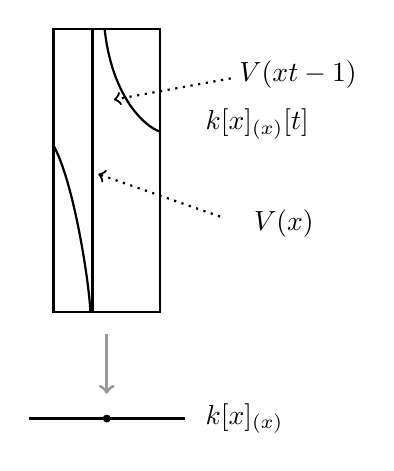
\begin{tikzpicture}[scale=0.9,line width=0.8pt]
  \draw (0,0) rectangle (1.5,4);
  \draw (0.55,0) -- (0.55,4);
  \draw (0.72,4) .. controls (0.82,3.05) and (1.28,2.62) .. (1.5,2.55);
  \draw (0,2.35) .. controls (0.28,1.85) and (0.5,0.45) .. (0.52,0);
  \node at (3.45,3.35) {$V(xt-1)$};
  \draw[dotted,->] (2.5,3.3) -- (0.85,3.0);
  \node at (3.25,1.25) {$V(x)$};
  \draw[dotted,->] (2.35,1.35) -- (0.63,1.95);
  \node[anchor=west] at (2.0,2.65) {$\Spec k[x]_{(x)}[t]$};
  \draw[gray!80,line width=1.1pt,->] (0.75,-0.3) -- (0.75,-1.15);
  \draw (-0.35,-1.5) -- (1.85,-1.5);
  \fill (0.75,-1.5) circle (1.6pt);
  \node[anchor=west] at (2.0,-1.5) {$\Spec k[x]_{(x)}$};
\end{tikzpicture}
\caption{\trSurface{} $\Spec k[x]_{(x)}[t]$ 上\trDimension{}与\trCodimension{}表现得古怪。（依原书手绘图重绘。）}\label{fig:codim-pathology}
\end{figure}

\textbf{12.3.14.}\ \hard\ \textbf{\trHypersurface{}上的直线，第 2 部分。}\quad （第 1 部分为 \S12.2.18。）现在我们给出\trKrull{}\trPrincipalIdealTheorem~12.3.3 的一个几何应用，借\mbox{练习~12.3.D(a)}加以施展。本小节全程在代数闭域 $\overline{k}$ 上工作。

\textbf{12.3.L.（练习）}
\begin{enumerate}[label=(\alph*)]
\item 设
\[
f(x_0,\dots,x_n)=f_d(x_1,\dots,x_n)+x_0f_{d-1}(x_1,\dots,x_n)+\cdots+x_0^{d-1}f_1(x_1,\dots,x_n)
\]
是一个齐次的 $d$ 次多项式（于是 $\deg f_i=i$），它在 $\mathbb{P}^n$ 中切出一张含 $p:=[1,0,\dots,0]$ 的\trHypersurface{} $X$。证明：存在过 $p$ 且含于 $X$ 的直线，当且仅当 $f_1=f_2=\cdots=f_d=0$ 在 $\mathbb{P}^{n-1}=\Proj\overline{k}[x_1,\dots,x_n]$ 中有公共零点。（提示：给定一个公共零点 $[a_1,\dots,a_n]\in\mathbb{P}^{n-1}$，证明连接 $p$ 与 $[0,a_1,\dots,a_n]$ 的直线含于 $X$。）
\item 若 $d\le n-1$，证明：过 $X$ 的任何一点 $p$，都有含于 $X$ 的直线。提示：\mbox{练习~12.3.D(a)}。
\item 若 $d\ge n$，证明：对 $\mathbb{P}^n$ 中「大多数」次数 $d$ 的\trHypersurface{} $X$（意即：凡其对应的点在参数空间 $\mathbb{P}^{\binom{n+d}{d}-1}$ 中落在某个非空\trZariski\trOpenSet{}内的\trHypersurface——参看注记~4.5.3 与\mbox{练习~9.3.J}——都算），「大多数点 $p\in X$」（即 $X$ 的某个非空稠密\trZariski\trOpenSet{}中的全部点）都没有 $X$ 中的直线经过。（提示：先证明存在单独某个 $X$ 中单独一点 $p$，没有任何直线经过它。\trChevalley{}定理~8.4.2 或许可派上用场。）
\end{enumerate}

\textbf{12.3.15.}\ \emph{\trhRemark{}。}\quad 射影（或\trProper）的 $k$-\trVariety{} $X$ 称为\textbf{\trUniruled}的（uniruled），若每一点 $p\in X$ 都含于某个 $\mathbb{P}^1\subset X$。（这个词出了本注记我们就不用了。）(b) 表明：所有次数至多为 $n-1$ 的\trHypersurface{}都是\trUniruled{}的。我们还能证明（要用到超出我们现有所知的方法；见 [Ko1, Cor.~IV.1.11]）：若 $\operatorname{char}\overline{k}=0$，则 $\mathbb{P}^n_k$ 中每张次数至少为 $n+1$ 的\trSmooth\trHypersurface{}都\emph{不}是\trUniruled{}的（这就把 (c) 中的那个开集显式化了）。此外，次数恰为 $n$ 的\trSmooth\trHypersurface{}\emph{确}是\trUniruled{}的，只是覆盖它的是二次曲线而非直线。于是，\trHypersurface{}的行为随着其次数相对 $n+1$ 的位置而有强烈的不同；这一点在许多别的方面也同样成立。次数小于 $n+1$ 的\trSmooth\trHypersurface{}是 \emph{Fano} \trVariety{}的例子；次数为 $n+1$ 的\trSmooth\trHypersurface{}是 \emph{Calabi--Yau} \trVariety{}的例子（依定义之不同，$n=1$ 的情形可能例外）；而次数大于 $n+1$ 的\trSmooth\trHypersurface{}则是\emph{一般型}（general type）\trVariety{}的例子。这些术语我们将在 \S21.5.5 中定义。
